% Hardware, connections, and software of the Day 1 lab.
\begin{frame}{Hardware and software}
  \begin{columns}[T]
    \begin{column}{0.47\textwidth}
      \textbf{Hardware for each group}
      \begin{itemize}
        \item XIAOML Kit: the XIAO ESP32S3 Sense with the camera, and the
              expansion board with the IMU and the display.
        \item USB-C data cable. A cable for charging only does not work.
        \item Wi-Fi antenna of the kit.
        \item Laptop: Windows, macOS, or Linux.
      \end{itemize}
    \end{column}
    \begin{column}{0.49\textwidth}
      \textbf{Software}
      \begin{itemize}
        \item Arduino IDE 2.
        \item Board core: esp32 by Espressif Systems 3.3.12.
        \item Library Seeed Arduino LSM6DS3 2.0.7 (IMU).
        \item Library U8g2 2.36.19 (display).
        \item Python 3.10 or later with \code{torch}, \code{torchvision},
              \code{numpy}, \code{matplotlib}, and \code{jupyterlab}.
      \end{itemize}
    \end{column}
  \end{columns}
  \vskip 0.8em
  \small
  \renewcommand{\arraystretch}{1.2}
  \begin{tabular}{@{}ll@{}}
    Lab files      & \code{Labs/day01/} \\
    Setup steps    & \code{Labs/SETUP.md} \\
    Tool versions  & \code{Labs/VERSIONS.md} \\
  \end{tabular}
\end{frame}

\begin{frame}{The kit has two boards and no wires}
  \begin{columns}[T]
    \begin{column}{0.30\textwidth}
      \centering
      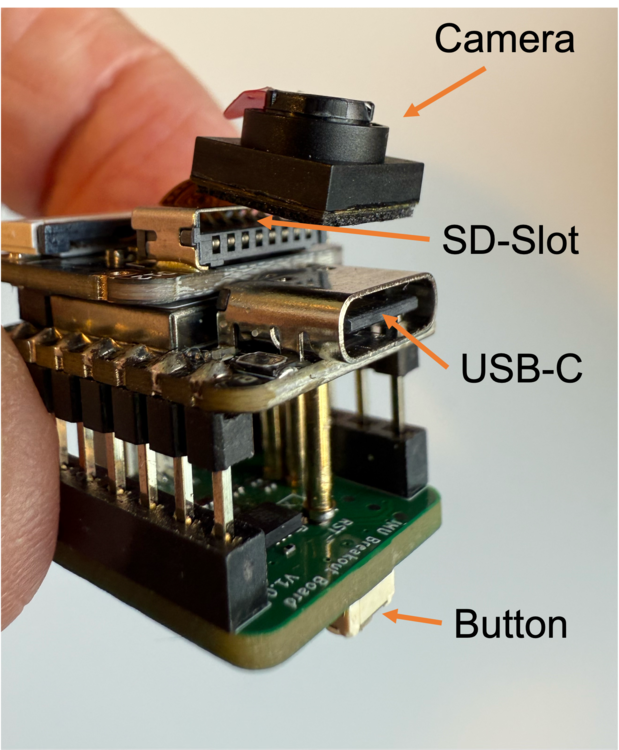
\includegraphics[height=3.5cm]{images/day01/kit-mounted.png}
    \end{column}
    \begin{column}{0.66\textwidth}
      \centering
      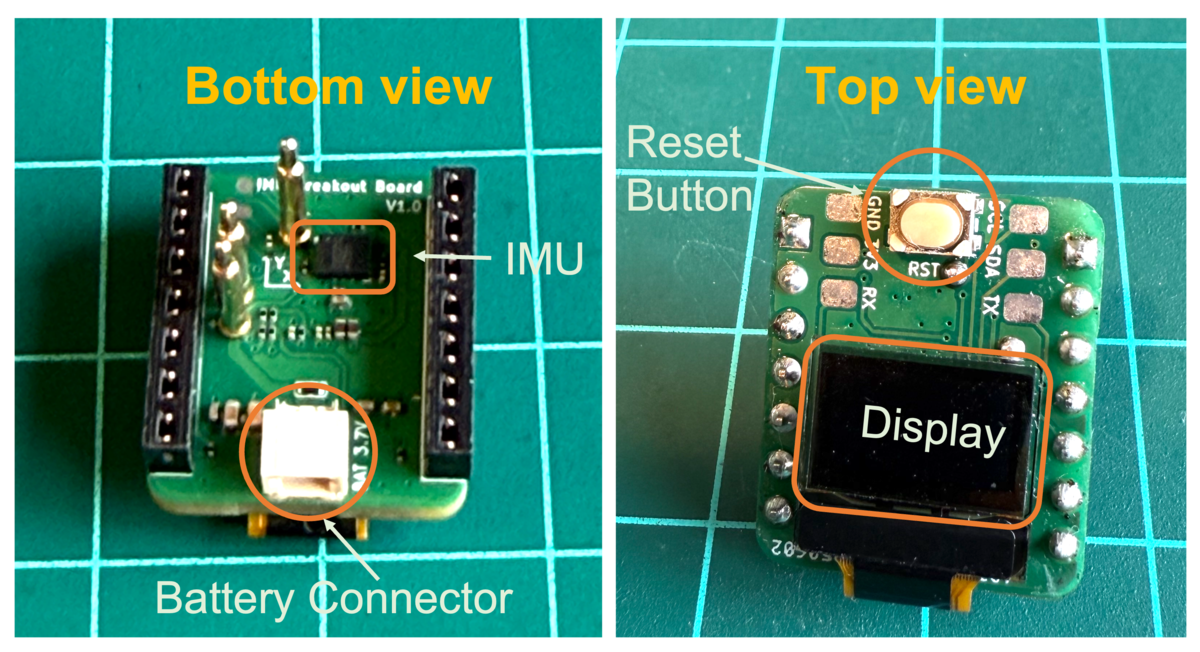
\includegraphics[height=3.3cm]{images/day01/expansion-board-views.png}
    \end{column}
  \end{columns}
  \vskip 0.2em
  \small
  \begin{itemize}
    \item The XIAO sits on the expansion board. You connect no wire.
    \item The expansion board has the IMU (I2C address 0x6A), the display
          (I2C address 0x3C), and the reset button.
    \item Connect the USB-C cable to the XIAO. The cable gives power and the
          serial port.
    \item Do not install the heat sink. It does not fit under the expansion
          board.
  \end{itemize}
  \source{Photographs and data: XIAOML Kit setup chapter of \emph{Machine
    Learning Systems}.}
\end{frame}
